\subsection{Plasma oscillation}

\begin{frame}{Plasma oscillation}
    \begin{columns}
        \column{0.5\textwidth}
        
        \vspace{2mm}
        \begin{itemize}
            \item Permitivity:
        \end{itemize}
        \begin{equation*}
            \varepsilon (\omega) = \varepsilon_0 \left(1 -  \dfrac{\omega_P^2}{\omega^2 - j \gamma \omega } \right)
        \end{equation*}
        can be negative in low frequency, but the loss is very high.
        \vspace{5mm}
        \begin{itemize}
            \item Plasma frequency:
        \end{itemize}
        \begin{equation*}
            \omega_P^2 = \dfrac{ne^2}{\varepsilon_0 m}.
        \end{equation*}
        \column{0.5\textwidth}

        \begin{figure}
            \centering
            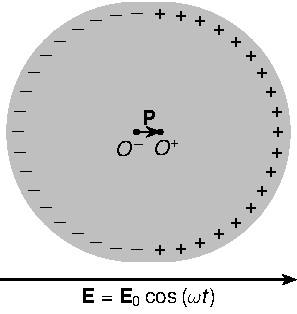
\includegraphics[width=\textwidth]{Figures/Rayleigh_scattering.pdf}
            \caption{Plasma oscillation}
            \label{fig:Plasma oscillation}
        \end{figure}
    \end{columns}
\end{frame}